%----------------------------------------------------------------------------------------
% Appendix
%----------------------------------------------------------------------------------------

\section{Appendices}
\label{chap:appendix}

\subsection{Appendix A: List of Figures}
\label{sec:appendixA}

\begin{figure}[h!]
  \centering
  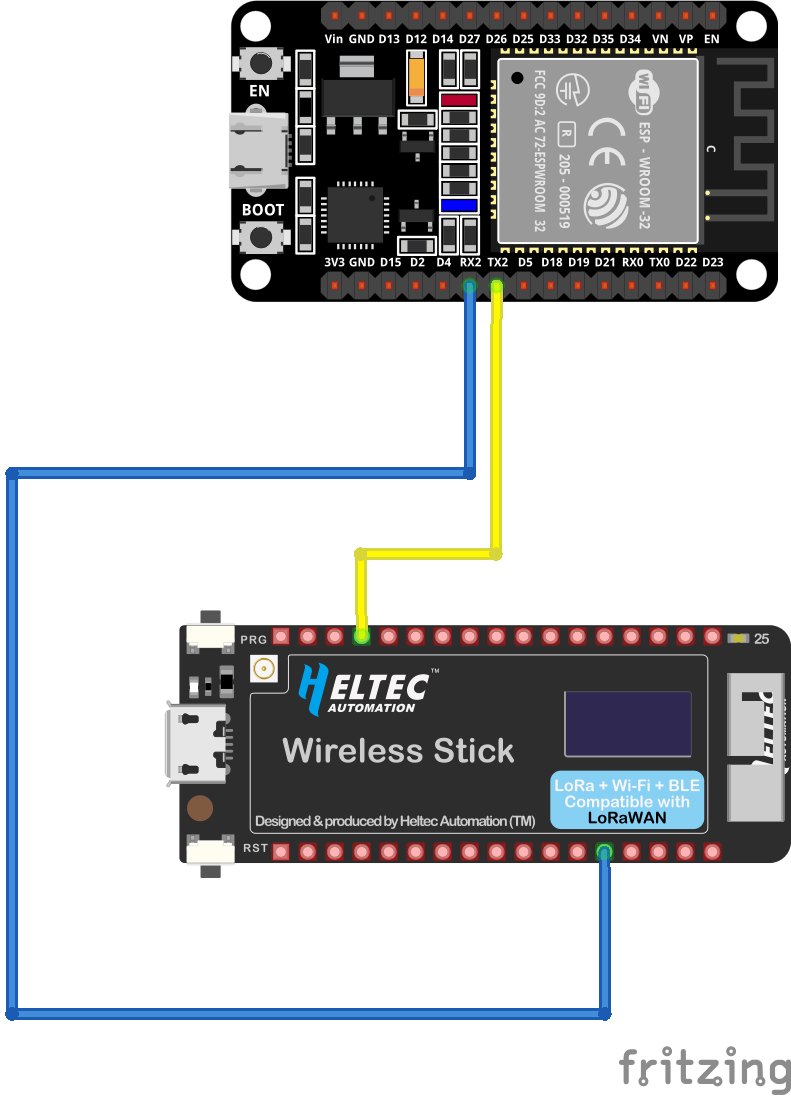
\includegraphics[width=0.8\linewidth]{figures/uart_connection.png}
  \caption{UART connection scheme}
  \label{fig:uart_connection}
\end{figure}

\begin{figure}[h!]
  \centering
  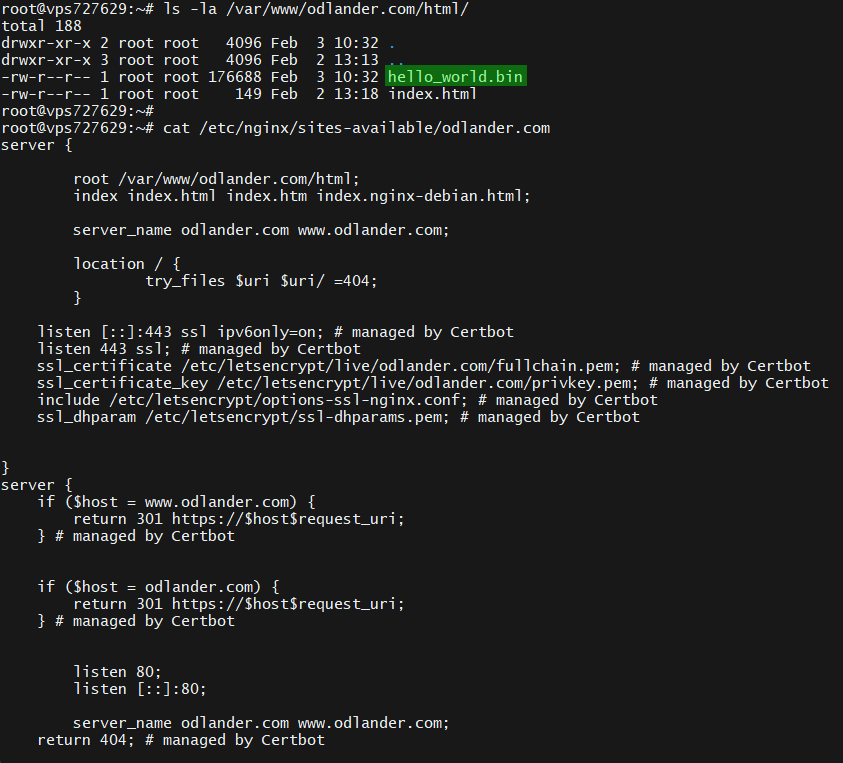
\includegraphics[width=0.8\linewidth]{figures/web_server.png}
  \caption{Web server}
  \label{fig:web_server}
\end{figure}


\begin{figure}[h!]
  \centering
  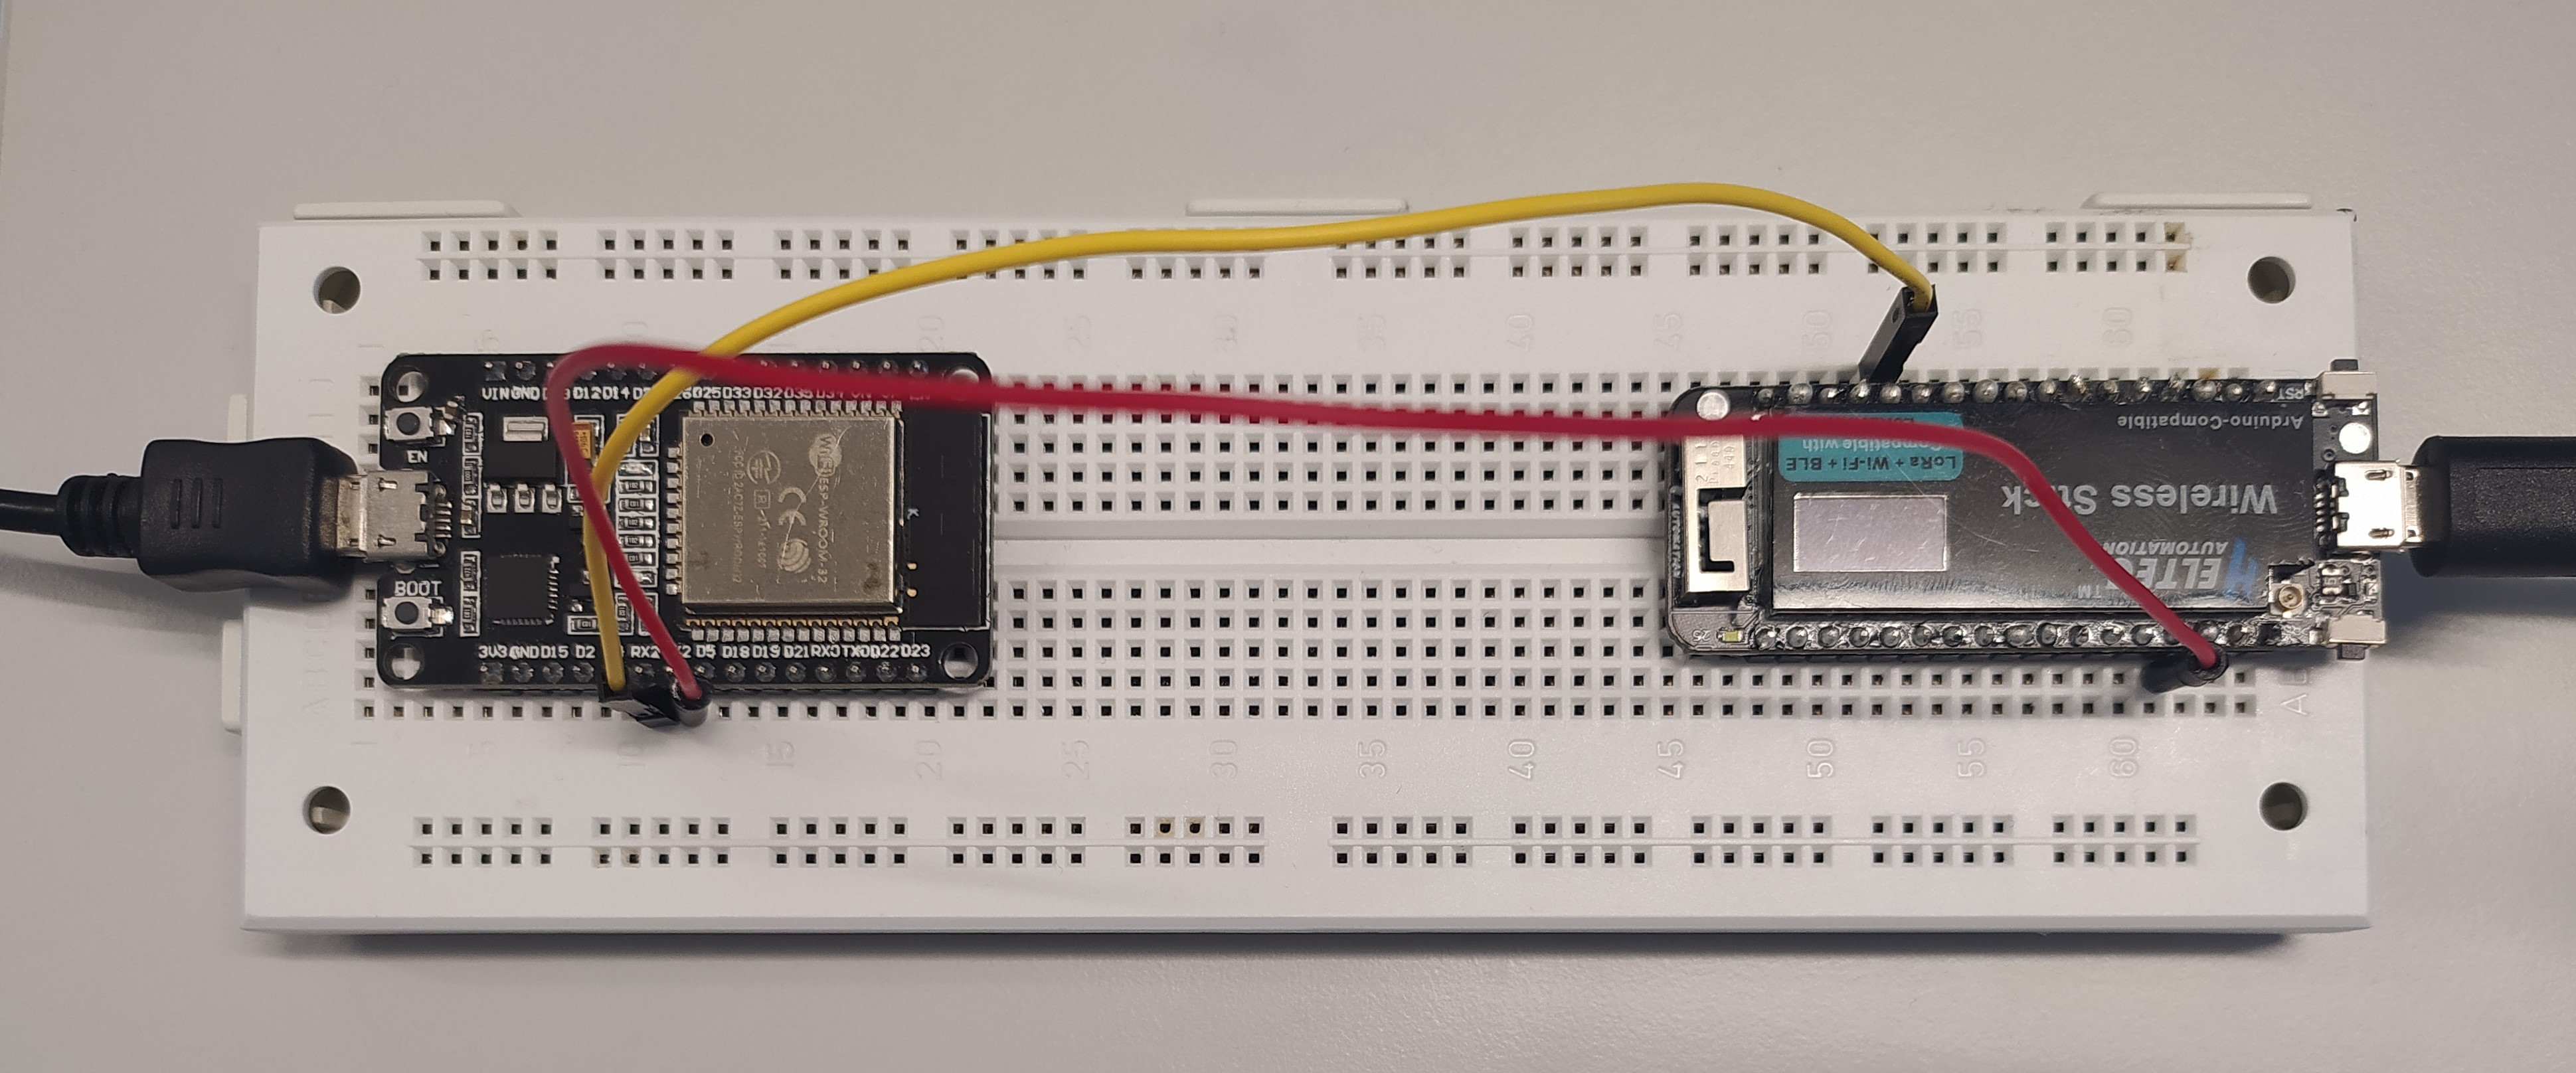
\includegraphics[width=0.8\linewidth]{figures/serial_connection.jpg}
  \caption{ESP32 connected via serial}
  \label{fig:serial_connection}
\end{figure}

\begin{figure}[h!]
  \centering
  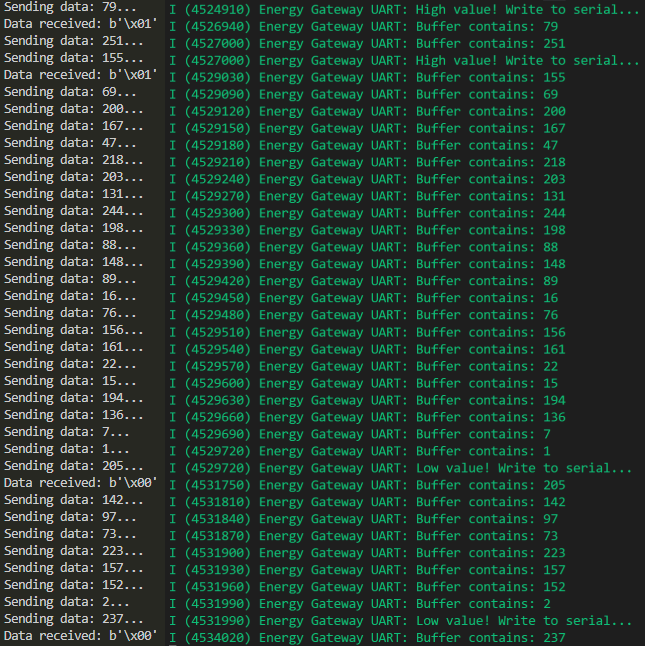
\includegraphics[width=0.8\linewidth]{figures/send_receive_33Hz.png}
  \caption{Serial communication at 33Hz}
  \label{fig:serial_communication_33hz}
\end{figure}

\begin{figure}[h!]
  \centering
  \begin{lstlisting}[style=CStyle]
    uart_read_bytes(
      ECHO_UART_PORT_NUM, 
      (char *) uartData, 
      UART_BUF_SIZE - 1, 
      20 / portTICK_PERIOD_MS 
      );
  \end{lstlisting}
  \caption{uart\_read\_bytes() function call}
  \label{fig:uart_read_bytes_function}
\end{figure}

\clearpage

\subsection{Appendix B: List of Tables}
\label{sec:appendixB}

\begin{table}[h!]
  \centering
  \caption{Task priority levels}
  \label{table:task-priorities}
  \begin{tabularx}{\textwidth}{p{1cm}Xp{10cm}}
    \hline
    \textbf{Priority} & \textbf{Example task} & \textbf{Description} \\ 
    \hline
    0 & \texttt{IDLE} & Idle tasks. \\
    \hline
    1 & \texttt{app\_main} & These are the tasks we prioritize the least.\\
    \hline
    2 & \texttt{ota\_task} & Tasks in this priority are prioritized very low.\\
    \hline
    18 & \texttt{tcpip\_task} & Important border. Tasks with higher priority than this can not be guaranteed to perform network operations as its possible they will override the TCP/IP stack. \\
    \hline
    19 & \texttt{uart\_task} & Using priority 19 or higher will guarantee an application task can run on Core 1 without being preempted by any built-in task\cite{espressif:esp-idf-programming-guide}. \\
    \hline
    20 & \texttt{event\_task} & The event handling system task to manage the default system event loop and execute callbacks. \\
    \hline
    22 & \texttt{esptimer\_task} & High Resolution Timer (ESP Timer) system task to manage high precision timer events and execute callbacks. \\
    \hline
    25 & \texttt{none} & Max Priority \\
    \hline
  \end{tabularx}
\end{table}
